\renewcommand{\theequation}{\theenumi}
\begin{enumerate}[label=\arabic*.,ref=\thesubsection.\theenumi]
\numberwithin{equation}{enumi}

\item \begin{align}
\begin{bmatrix}x & y\end{bmatrix}\begin{bmatrix}A & \frac{B}{2}\\\frac{B}{2} & C\end{bmatrix}\begin{bmatrix}x \\ y\end{bmatrix} + \begin{bmatrix}D & E\end{bmatrix}\begin{bmatrix}x & y\end{bmatrix} +F
\end{align}

\item
\begin{align}
\begin{bmatrix}\vec x\end{bmatrix}^T\begin{bmatrix}1 & 0\\0 & 0\end{bmatrix}\begin{bmatrix}\vec x\end{bmatrix} + \begin{bmatrix}-2 & 0\end{bmatrix}\begin{bmatrix}\vec x\end{bmatrix} -8
\\
x^2-2x-8 = 0
\\
\left(x-4\right)\left(x+2\right) = 0
\\
\vec s_1 = 4 ,\vec s_2 =-2 
\end{align}
\begin{figure}[!ht]
	\centering
	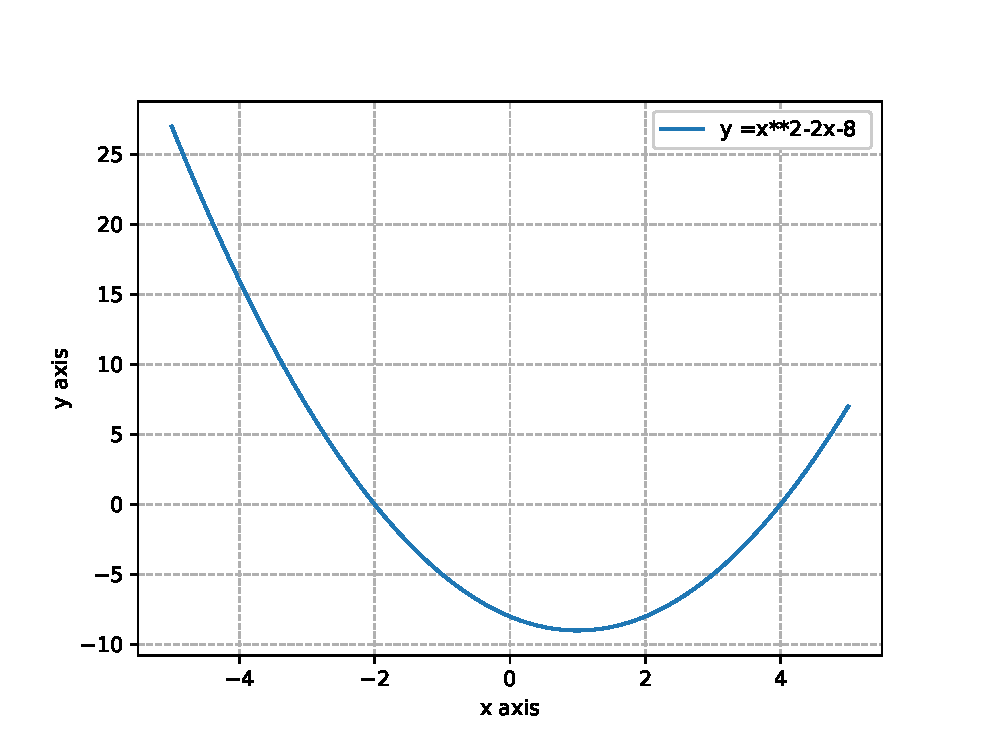
\includegraphics[width=\columnwidth]{./figures/perabola1.eps}
	\caption{equation 1 }
	\label{fig:perabola1}
\end{figure}
\begin{lstlisting}
codes/perabola2.py
\end{lstlisting}



\item
\begin{figure}[!ht]
	\centering
	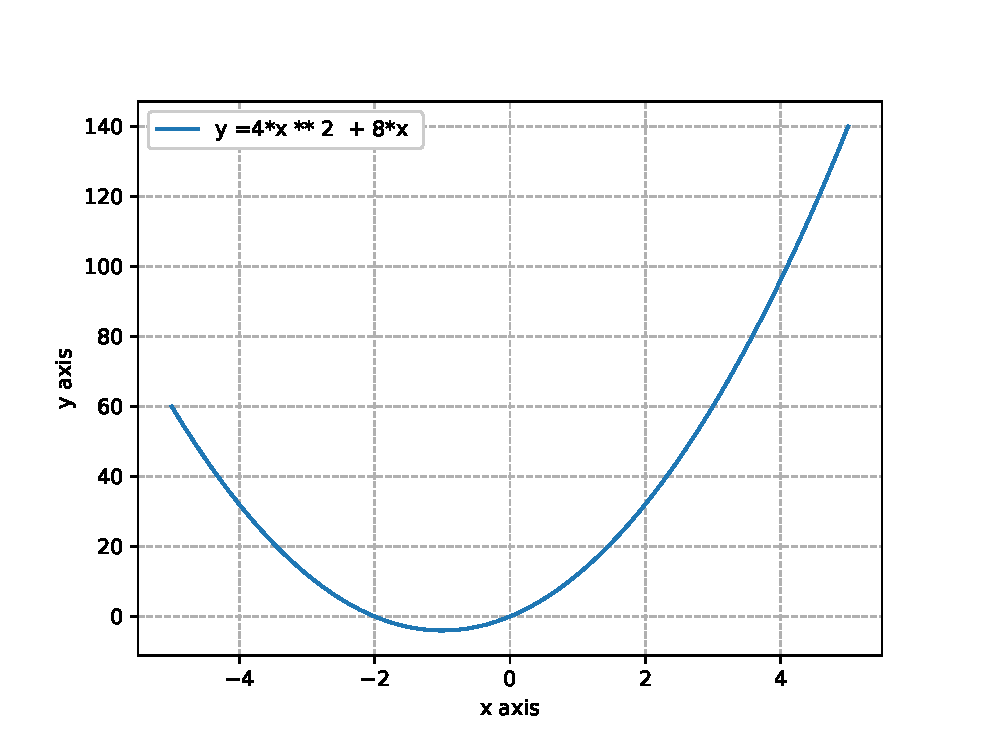
\includegraphics[width=\columnwidth]{./figures/perabola2.eps}
	\caption{equation 2 }
	\label{fig:perabola2}
\end{figure}
\begin{lstlisting}
codes/perabola2.py
\end{lstlisting} 
\begin{align}
\begin{bmatrix}\vec x\end{bmatrix}^T\begin{bmatrix}4 & 0\\0 & 0\end{bmatrix}\begin{bmatrix}\vec x\end{bmatrix} + \begin{bmatrix}8 & 0\end{bmatrix}\begin{bmatrix}\vec x\end{bmatrix} 
\\
4u^2 + 8u = 0
\\
\left(4u\right)\left(u+2\right) = 0
\\
\vec u_1 = 0 ,\vec u_2 =-2 
\end{align}



\item
\begin{align}
\begin{bmatrix}\vec x\end{bmatrix}^T\begin{bmatrix}4 & 0\\0 & 0\end{bmatrix}\begin{bmatrix}\vec x\end{bmatrix} + \begin{bmatrix}-4 & 0\end{bmatrix}\begin{bmatrix}\vec x\end{bmatrix} +1
\\
4s^2-4s+1 = 0
\\
\left(2s-1\right)\left(2s + 1\right) = 0
\\
\vec s_1 = \frac{1}{2} ,\vec s_2 =-\frac{1}{2} 
\end{align}
\begin{figure}[!ht]
	\centering
	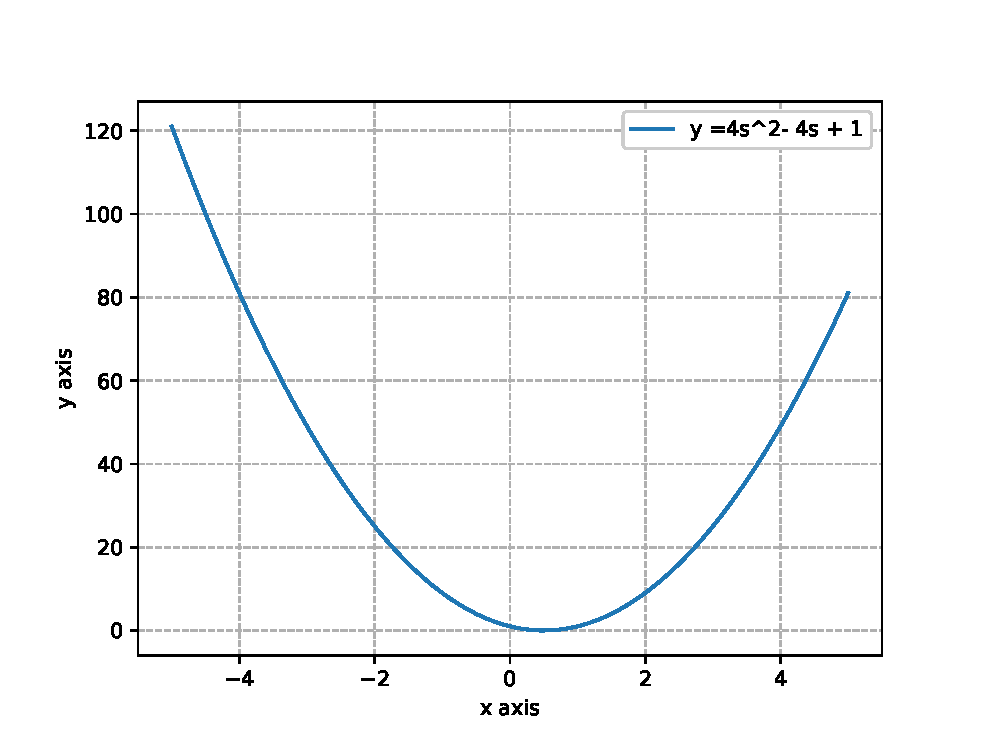
\includegraphics[width=\columnwidth]{./figures/perabola3.eps}
	\caption{equation 3 }
	\label{fig:perabola3}
\end{figure}
\begin{lstlisting}
codes/perabola3.py
\end{lstlisting}


	\item
\begin{align}
\begin{bmatrix}\vec x\end{bmatrix}^T\begin{bmatrix}1 & 0\\0 & 0\end{bmatrix}\begin{bmatrix}\vec x\end{bmatrix} + \begin{bmatrix}0 & 0\end{bmatrix}\begin{bmatrix}\vec x\end{bmatrix} -15
\\
t^2 - 15 = 0
\\
\vec t_1 = \sqrt {15} ,\vec t_2 =-\sqrt {15} 
\end{align}
\begin{figure}[!ht]
	\centering
	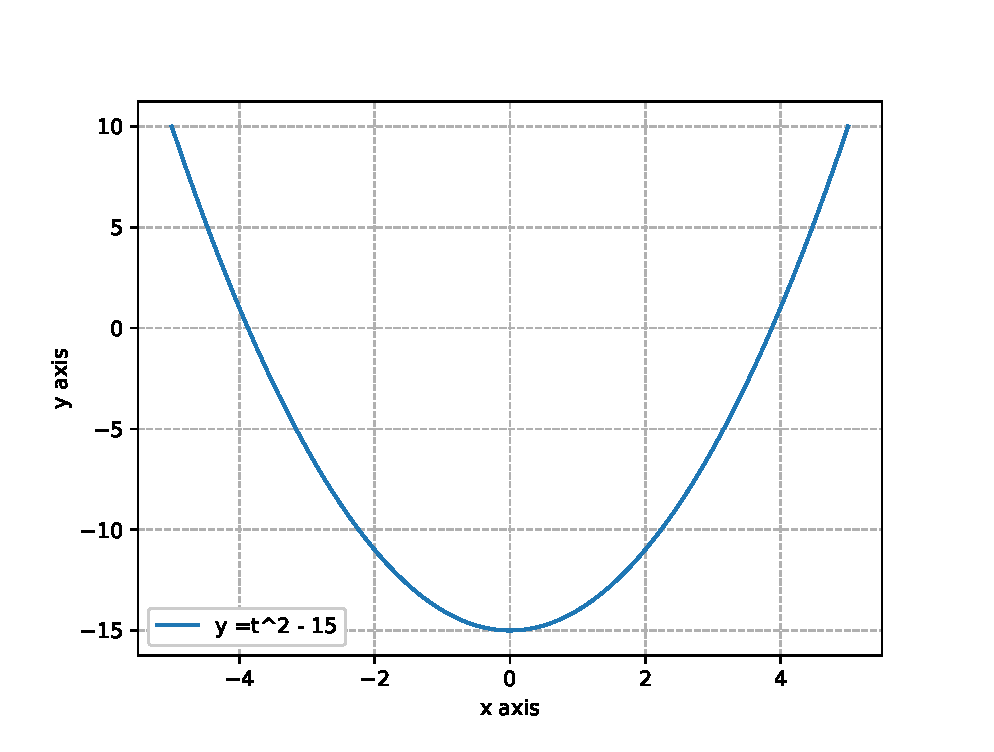
\includegraphics[width=\columnwidth]{./figures/perabola4.eps}
	\caption{equation 4 }
	\label{fig:perabola4}
\end{figure}
\begin{lstlisting}
codes/perabola4.py
\end{lstlisting}



\item
\begin{align}
\begin{bmatrix}\vec x\end{bmatrix}^T\begin{bmatrix}6 & 0\\0 & 0\end{bmatrix}\begin{bmatrix}\vec x\end{bmatrix} + \begin{bmatrix}-7 & 0\end{bmatrix}\begin{bmatrix}\vec x\end{bmatrix} -3
\\
6x^2-3-7x = 0
\\
\left(2x - 3\right)\left(3x\ + 1\right) = 0
\\
\vec x_1 = \frac{3}{2},\vec x_2 =-\frac{1}{3}
\end{align}
\begin{figure}[!ht]
	\centering
	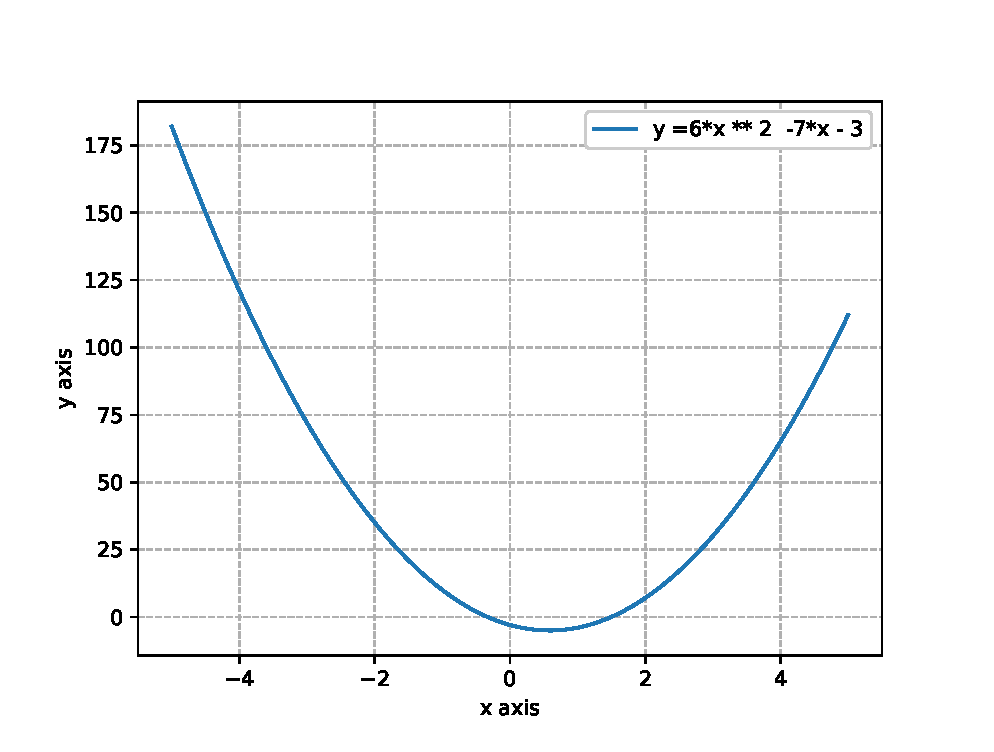
\includegraphics[width=\columnwidth]{./figures/perabola5.eps}
	\caption{equation 5 }
	\label{fig:perabola5}
\end{figure}
\begin{lstlisting}
codes/perabola5.py
\end{lstlisting}


\item
\begin{align}
\begin{bmatrix}\vec x\end{bmatrix}^T\begin{bmatrix}3 & 0\\0 & 0\end{bmatrix}\begin{bmatrix}\vec x\end{bmatrix} + \begin{bmatrix}-1 & 0\end{bmatrix}\begin{bmatrix}\vec x\end{bmatrix} -4
\\
3x^2-2x-8 = 0
\\
\left(3x 44\right)\left(x + 1\right) = 0
\\
\vec x_1 = -1,\vec x_2 =-\frac{4}{3}
\end{align}
\begin{figure}[!ht]
	\centering
	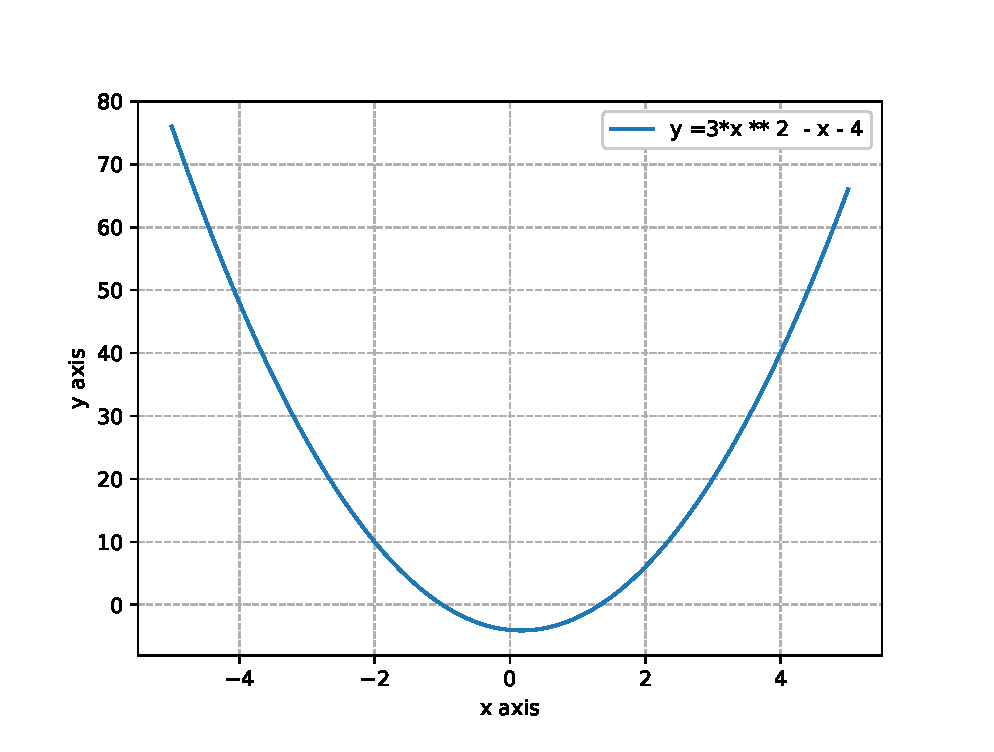
\includegraphics[width=\columnwidth]{./figures/perabola6.eps}
	\caption{equation 6 }
	\label{fig:perabola6}
\end{figure}
\begin{lstlisting}
codes/perabola6.py
\end{lstlisting}

\end{enumerate}